\documentclass{article}
\usepackage[utf8]{inputenc}
\usepackage{geometry}
\usepackage{tabularx}
\usepackage{hyperref}
\usepackage{graphicx}
\usepackage{adjustbox}
\usepackage{multicol}
\usepackage{caption}
\usepackage{subcaption}
\usepackage{xurl}
\usepackage{wrapfig}
\usepackage{float}
\usepackage{enumitem}
\usepackage{makecell}
\usepackage{amsmath}
\usepackage{tikz}

\geometry{
 a4paper,
 total={170mm,257mm},
 left=20mm,
 top=20mm,
 }

\usetikzlibrary{shapes.geometric, arrows}

\title{}
\author{\textbf{Author}\\Rosalie de Winther (1326236)\\\\\textbf{Company supervisor}\\Jacco Bikker\\\\\textbf{Primary supervisor}\\Alex Telea\\\\\textbf{Secondary supervisor}\\Peter Vangorp}
\begin{document}
\begin{titlepage}
    \begin{center}
        \vspace*{1cm}

        \textbf{\huge Volumetric data structures for real-time ray tracing}

        \vspace{1cm}

        \large Game and Media Technology\\
        Master thesis


        \vspace{1cm}

        \includegraphics[width=\textwidth]{figures/disney _cloud.png}

        \vspace{1cm}



        \vspace{1cm}

        \raggedright \textit{Author:} Rosalie de Winther (1326236)\\
        \textit{Company supervisor:} Jacco Bikker\\
        \textit{Primary supervisor:} Alex Telea\\
        \textit{Secondary supervisor:} Peter Vangorp\\
        \today

    \end{center}
\end{titlepage}



\clearpage
\section*{Abstract} \label{abstract}
Volumetric effects such as clouds, explosions, smoke, and fog are important scene elements for computer games. While these can be efficiently handled in a rasterizer, path tracers typically struggle to render them efficiently. In this thesis we provide the required prior knowledge to think about the different trade-offs of volume data structures, and we provide a specialized implementation for compressed density data. The resulting data structure reduces the voxel data memory footprint by a factor of 8 to 16 times over 16-bit floating point values. This is achieved by utilizing a novel method of storing density data in block-compressed textures and deduplicating homogeneous nodes. These methods allow us to store animation sequences in game-ready asset sizes and render them at real-time frame rates.
\clearpage
\section*{Acknowledgments} \label{acknowledgments}

Firstly I would like to thank Traverse Research for accommodating my research and providing incredible guidance. Secondly, I want to thank Jacco Bikker for inviting me to help organize High Performance Graphics 2023, and countless discussions about voxels, rendering and GPUs. Tertiary, I would like to thank Alex Telea for his very critical look at all the documents that I made during the past year and for always being able to help with any questions regarding my thesis, it was very helpful and taught me a lot. Fourthly, I want to thank Emilio Laiso for all the collaboration on the implementation side, and for integrating our two systems to allow for (in my opinion) very pretty renders. Furthermore, I would like to thank Manon Oomen for her support during my thesis and the nitty-gritty detailed explanations of GPU performance. And of course, I want to thank Devon Dissel for always being there to cheer me up and dealing with my long days away from home.

I also want to thank some communities that have helped me through the process of writing this thesis either on an emotional or technical level. Namely, The Revenant Rebellion for providing some distractions when stress was high. The VoxelGameDev.com community for providing technical help and staying up to date with the latest developments in volume data structure research. The study association Sticky for providing a comfortable space near the University to study and work. And lastly the Utrecht Skate Parade for keeping me fit throughout it all.
\clearpage
\tableofcontents
\clearpage
\section{Introduction} \label{introduction}
This thesis aims to be an introduction to volume rendering data structures as well as introduce two compression steps of volume density data. The focus is not so much on shrinking our geometry, but more so on shrinking the actual density data. This is required for our desire to implement full three-dimensional volume animation models in the in-house renderer at Traverse Research. A basic understanding of the Graphics processing unit (GPU) is expected. Along with knowledge of the basic terminology used when talking about ray tracing such as acceleration structures, primitives, rays, and the rendering equation.

The structure of this thesis is as follows. In Chapter \ref{related_work} we start with an introduction into rendering, volume rendering specifically and discuss some sparse volume data structures along with general compression techniques. In Chapter \ref{requirements} we go over the requirements set up by \href{https://traverseresearch.nl/}{Traverse Research} which were the main guidelines/constraints for this research. After which Chapter \ref{approach} follows where we cover the main techniques behind our implementation, which should convey the main idea behind the researched techniques.  The following chapter, Chapter \ref{implementation}, describes how our methods were implemented and used in Traverse's custom engine. This implementation led to multiple tests and benchmarks which are described in Chapter \ref{results}. And lastly we conclude this research in Chapter \ref{conclusion} where we answer the research questions and show some final renders made using our methods.


\subsection{Traverse Research} \label{introduction:traverse_research}
\href{https://traverseresearch.nl/}{Traverse Research} is a company that specialized in state-of-the-art research in graphics, and more specifically ray tracing. Traverse does research for multiple hardware vendors including AMD and ARM, for whom they develop ray tracing algorithms, optimizations, and workloads.
\subsubsection{Breda} \label{introduction:traverse_research:breda}
Traverse's current in-house hybrid rendering framework "Breda" includes many features that are expected from a modern renderer. However, volume rendering is still largely unexplored. Breda can compile for either a Vulkan or DirectX 12 backend to make use of the latest ray tracing features. Along with that, some advanced rendering techniques are used. Most notably bindless rendering\cite{BindlessRenderingSetup} and render graphs\cite{RenderGraph101}. The former is a different way of interfacing with data on the GPU, while the latter simplifies GPU synchronization while optimizing dispatch ordering based on read and write dependencies of different pieces of data on the GPU. All of this is written in Rust and HLSL.
\subsubsection{Volumes} \label{introduction:traverse_research:volumes}
In parallel to this research there is another project going on that focuses on shading as explained in Section \ref{related_work:path_traced_volume_rendering}. The combination of both projects allows for physically based shading of large animated volumetric effects in real-time. The exact placement of this research inside the Breda framework can be seen in Figure \ref{fig:project_structure}.

\begin{figure}[H]
    \centering
    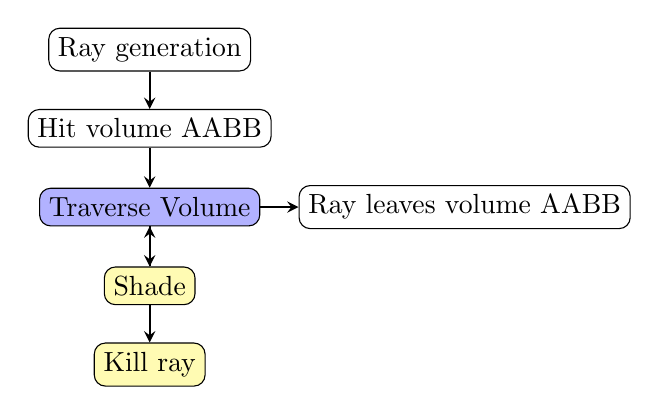
\begin{tikzpicture}[node distance=1cm]
        \tikzstyle{arrow} = [thick,->,>=stealth]
        \tikzstyle{done} = [rectangle, rounded corners, minimum width=1cm, minimum height=0.33cm,text centered, draw=black]
        \tikzstyle{this} = [rectangle, rounded corners, minimum width=1cm, minimum height=0.33cm,text centered, draw=black, fill=blue!30]
        \tikzstyle{other} = [rectangle, rounded corners, minimum width=1cm, minimum height=0.33cm,text centered, draw=black, fill=yellow!30]
        \node (start) [done] {Ray generation};
        \node (aabb) [done, below of=start] {Hit volume AABB};
        \node (trav) [this, below of=aabb] {Traverse Volume};
        \node (shade) [other, below of=trav] {Shade};
        \node (kill) [other, below of=shade] {Kill ray};
        \node (leaves) [done, right of=trav, xshift=3cm] {Ray leaves volume AABB};

        \draw [arrow] (start) -- (aabb);
        \draw [arrow] (aabb) -- (trav);
        \draw [arrow] (trav) -- (shade);
        \draw [arrow] (trav) -- (leaves);
        \draw [arrow] (shade) -- (trav);
        \draw [arrow] (shade) -- (kill);

    \end{tikzpicture}
    \caption{Flow diagram highlighting where this research fits inside the Breda framework. The white boxes indicate parts of the pipeline that already exist inside the Breda framework. The blue box shows what this research will focus on, and the yellow boxes highlight what parts were developed in parallel to this research. As can be seen, when rays bounce inside a volume, they can repeatedly be shaded and continue traversal until they either leave the volume or are killed because they won't contribute any light to the scene.}
    \label{fig:project_structure}
\end{figure}
\clearpage
\section{Requirements} \label{requirements}
This research focuses on a specific set of requirements having to do with volume data structures. We want to support volumetric animations in the Breda renderer developed by Traverse Research (as explained in section \ref{introduction:traverse_research}). This means that we want to support path tracing volumetric effects, with optional emission using assets that are proportional to standard game asset sizes. Below are the most important requirements our data structure should adhere to.
\subsection{Asset size} \label{requirements:asset_size}
Asset sizes in games have been growing for a while, with the latest titles shipping 4k textures. To keep our assets in line with standard game assets we should not be going above 100MB per volume animation. This requires both the volume geometry and attributes to be significantly compressed.
\subsection{Sampling speed} \label{requirements:sampling_speed}
Our 'random' access times should be fast enough to enable path-traced volumetrics on high-end current-generation hardware. In reality, 'random' access is never random \cite{museth2013vdb}, so optimizing cache utilization to improve spatially coherent access' will go a long way.
\subsection{Animation playback} \label{requirements:animation_playback}
Fast animation playback is the most novel part of this research. And if we are running high framerate animations these should not take up too much time of our frame budget. So complex expansive delta update schemes are not an option for us.
\subsection{Lossy compression} \label{requirements:lossy_compression}
Pretty much all effective compression schemes for floating point data are lossy in some form. The difficult task is making this lossiness as hard as possible to notice. So when we compress our volume data it is essential that we keep its high and low frequency features intact.
\subsection{Level of detail} \label{requirements:level_of_detail}
For certain parts of our rendering process, we need to use the absolute highest level of detail, for example for our primary rays. However, for our secondary or shadow rays, we do not have to care as much about the exact volume boundaries. This will allow us to use a lower level of detail model to achieve almost the same results, which in turn allows us to improve performance.

\clearpage
\section{Research questions}\label{research_questions}
\subsection{Optimal data structure}\label{research_questions:optimal_data_structure}
\subsection{Performance bottlnecks}\label{research_questions:performance_bottlenecks}

These requirements lead into the following research questions:\\

\noindent\textbf{What data structures, or combination of structures, are optimal for ray tracing, memory and animation, and can these structures be converted into each other?} We have already seen that there are different techniques which are optimized for different metrics. So if we know the optimal method for each of our requirements, we can work towards combining their strengths without having to create one structure which can do it all (which evidently does not exist, yet).

\noindent\textbf{Is volume traversal memory or compute bound?} This question should provide insight into future optimization techniques. Insight into questions like "if L1 cache size is increased by X amount, will this improve volume traversal speed?" or "if the clock speed of a GPU is increased, what will the impact on our volume traversal be?" will be acquired.


\clearpage
\section{Approach} \label{approach}
\subsection{VDB data structure} \label{approach:vdb_data_structure}
\subsection{Simulation} \label{approach:simulation}
\subsection{Flipbook animations} \label{approach:flipbook_animations}
\subsection{Texture compression} \label{approach:texture_compression}
\subsection{Clustering similar nodes} \label{approach:clustering_similar_nodes}
\clearpage
\section{Implementation} \label{implementation}
\subsection{Asset pipeline} \label{implementation:asset_pipeline}
\subsection{Shaders} \label{implementation:shaders}
\subsection{Texture formats} \label{implementation:texture_formats}
\subsection{Libraries} \label{implementation:libraries}
\clearpage
\section{Results} \label{results}

\subsection{Models} \label{results:models}
Multiple models were used to evaluate the implemented methods in section \ref{implementation}. The model with the largest scale is the Disney cloud \cite{DisneyCloud}. Our implementation is bound by volumes with size $4096^3$ so we use the half resolution version. We also use multiple models from the \href{https://www.openvdb.org/download/}{OpenVDB website} and the \href{https://jangafx.com/software/embergen/download/free-vdb-animations/}{JangaFX website}. A mix of models was used with diverse axis size, number of voxels, animation frame number and shapes. 

\begin{table}[htbp]
    \centering 
    \begin{tabularx}{\textwidth}{|X|c|c|c|c|}
    \hline
    \textbf{Dataset} & \textbf{Voxels} & \textbf{Dimensions} & \textbf{Animation frames} & \textbf{Render}\\
    \hline
    \textbf{fire} & 4,458,790 & [160, 363, 152] & 1 & \includegraphics[width=4cm]{figures/disney _cloud.png}\\
    \hline
    \textbf{bunny} & 5,513,993 & [627, 620, 488] & 1 & \includegraphics[width=1cm]{figures/disney _cloud.png}\\
    \hline
    \textbf{bunny cloud} & 19,210,271 & [576, 571, 437] & 1 & \includegraphics[width=1cm]{figures/disney _cloud.png}\\
    \hline
    \textbf{armadillo} & 22,734,512 & [1,275, 1,518, 1,159] & 1 & \includegraphics[width=1cm]{figures/disney _cloud.png}\\
    \hline
    \textbf{dragon} & 23,347,893 & [2,022, 910, 1,346] & 1 & \includegraphics[width=1cm]{figures/disney _cloud.png}\\
    \hline
    \textbf{cloud pack} & 49,869,596 & [349, 178, 530] & 10 & \includegraphics[width=1cm]{figures/disney _cloud.png}\\
    \hline
    \textbf{disney cloud} & 188,358,293 & [993, 675, 1,224] & 1 & \includegraphics[width=1cm]{figures/disney _cloud.png}\\
    \hline
    \textbf{chimney} & 239,747,485 & [160, 350, 505] & 100 & \includegraphics[width=1cm]{figures/disney _cloud.png}\\
    \hline
    \textbf{shockwave} & 631,494,157 & [732, 140, 729] & 50 & \includegraphics[width=1cm]{figures/disney _cloud.png}\\
    \hline
    \end{tabularx}
    \caption{Data Summary}
    \label{tab:data-summary}
\end{table}


\subsection{Tree size} \label{results:tree_size}
As described in section \ref{approach:flipbook_animations}, we put our focus on compressing the voxel data instead of our tree structure size. This results in long animation sequences having large trees.  

\begin{table}[htbp]
    \centering
    \caption{Data Summary}
    \label{tab:data-summary}
    \begin{tabularx}{\textwidth}{|c|c|c|c|c|c|c|c|c|}
    \hline
    \textbf{Dataset} & \textbf{Total Voxels} & \textbf{Axis Sizes} & \textbf{L1 Nodes} & \textbf{L2 Nodes} & \textbf{L3 Nodes} & \textbf{Bricks} & \textbf{Total Size} \\
    \hline
    \textbf{fire} & 4,458,790 & [160, 363, 152] & 1 & 32,768 & 65,536 & 65,536 & 28MB & 1 \\
    \hline
    \textbf{bunny} & 5,513,993 & [627, 620, 488] & 1 & 32,768 & 307,200 & 65,536 & 46MB & 1 \\
    \hline
    \textbf{bunny cloud} & 19,210,271 & [576, 571, 437] & 1 & 32,768 & 303,104 & 131,072 & 54MB & 1 \\
    \hline
    \textbf{armadillo} & 22,734,512 & [1,275, 1,518, 1,159] & 1 & 32,768 & 1,339,392 & 131,072 & 125MB & 1 \\
    \hline
    \textbf{dragon} & 23,347,893 & [2,022, 910, 1,346] & 1 & 32,768 & 1,302,528 & 131,072 & 122MB & 1 \\
    \hline
    \textbf{cloud pack} & 49,869,596 & [349, 178, 530] & 10 & 327,680 & 905,216 & 196,608 & 255MB & 10 \\
    \hline
    \textbf{disney cloud} & 188,358,293 & [993, 675, 1,224] & 1 & 32,768 & 1,007,616 & 327,680 & 127MB & 1 \\
    \hline
    \textbf{chimney} & 239,747,485 & [160, 350, 505] & 100 & 3,276,800 & 9,195,520 & 917,504 & 2.434GB & 100 \\
    \hline
    \textbf{shockwave} & 631,494,157 & [732, 140, 729] & 50 & 1,638,400 & 9,658,368 & 1,900,544 & 1.746GB & 50 \\
    \hline
    \end{tabularx}
\end{table}

\subsection{Block compression} \label{results:block_compression}

\begin{figure}[H]
    \centering
    %\subfloat[]{
    %    \includegraphics[width=0.45\textwidth]{}
    %}
    %\hfill
    %\subfloat[]{
    %    \includegraphics[width=0.45\textwidth]{}
    %}

    \caption{} \label{fig:implementation:compression:bc}
\end{figure}
\subsection{Clustering} \label{results:clustering}


\begin{figure}[H]
    \centering
    \subfloat[]{
        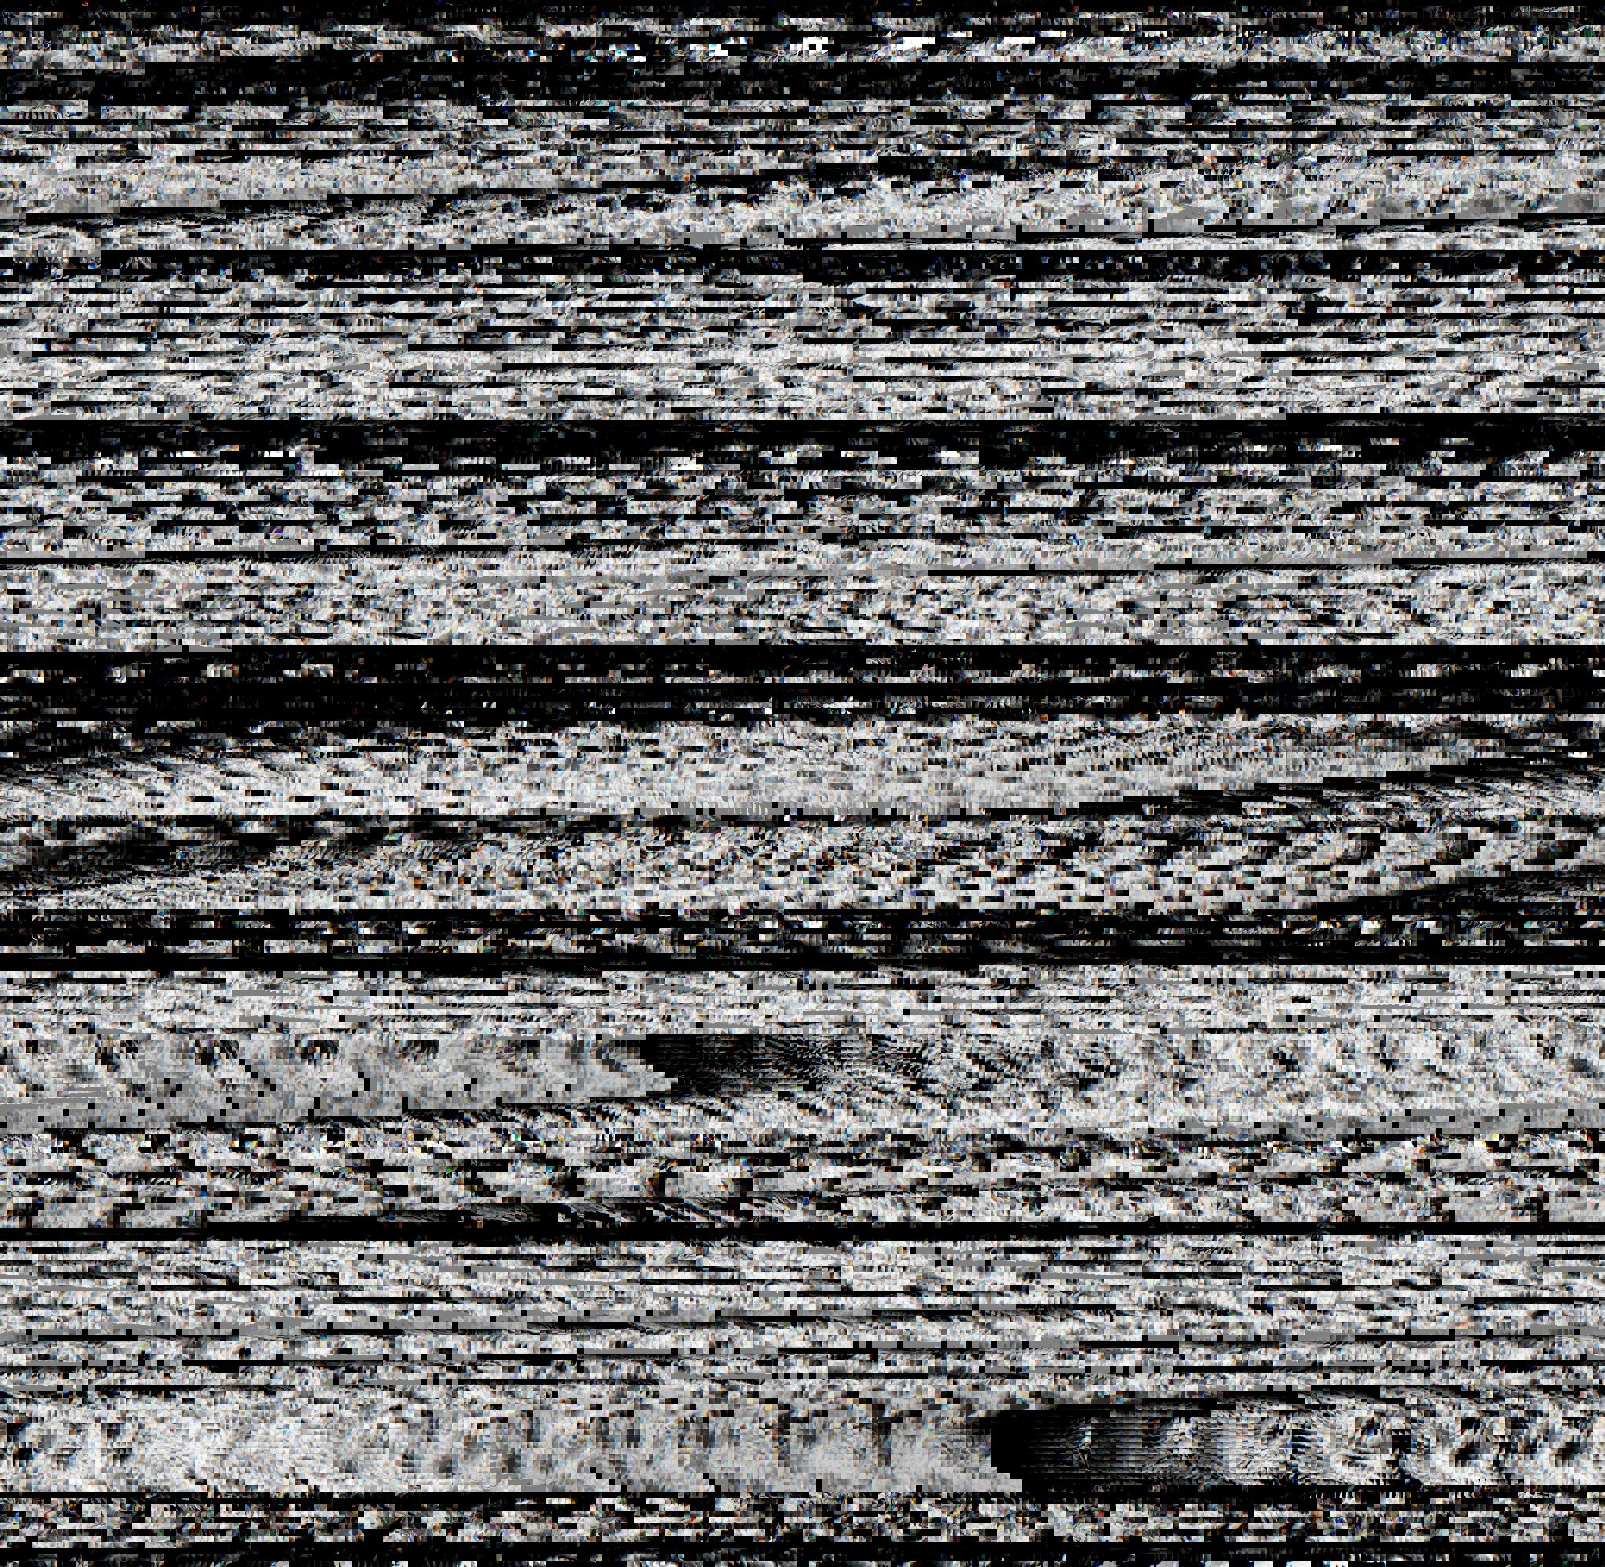
\includegraphics[width=0.45\textwidth]{figures/pre_clustered_memory.png} \label{fig:implementation:compression:pre_cluster}
    }
    \hfill
    \subfloat[]{
        
\includegraphics[width=0.45\textwidth]{figures/post_clustered_memory.png} \label{fig:implementation:compression:post_cluster}
    }
    \caption{The results of our clustering compression technique. All of these results use Bc7 encoding. Figure \ref{fig:implementation:compression:pre_cluster} shows a slice out of the voxel brick data texture on the GPU. There are visible long chains of black or otherwise greyscale slices which means that these bricks are mostly homogeneous inside that brick. In Figure \ref{fig:implementation:compression:post_cluster} we again see a slice of the voxel brick data texture, but this time after running our clustering algorithm. There are visibly fewer patches greyscale bricks when compared to figure \ref{fig:implementation:compression:pre_cluster}. This shows us that we are actually removing bricks which are homogeneous, and keeping unique nodes.} \label{fig:implementation:compression:cluster}
\end{figure}
\clearpage
\section{Conclusion} \label{conclusion}


\subsection{Future research} \label{conclusion:future_research}

\begin{itemize}
    \item One point of improvement to this technique could be a more optimized rejection scheme. Currently, we reject if the normalized variance of all brick values is too high. This only allows us to cluster homogeneous bricks, and not brick which contain a smooth gradient, even though there are bricks which are simply a gradient in one specific axis which likely could be clustered. Another major issue with this compression scheme is the build times. It currently takes multiple minutes to compress both the shockwave and the chimney animation, which makes development iteration times very slow.
    \item Different texture compression schemes can be experimented with. Certain platforms, like mobile, have different texture compression formats namely, Ericsson Texture Compression (ETC) and Adaptive scalable compression (ASTC). ETC has 1 bit per voxel which is twice the compression ratio of the method described in \ref{approach:texture_compression}. And ASTC can compress between $0,15$ and $1,19$ depending on certain options. These compression schemes will change the quality of our data, but might be worth it on the supported platforms.
    \item Different tree topologies can be experimented with. Most notably B+Tree's with uniform layer sizes. This might make it possible to deduplicate many of the bit masks and thus shrink the tree size. Another benefit as mentioned in \cite{hoetzlein2016gvdb}. By using a tree where all internal nodes are $8^3$ we get better ray tracing performance.
    \item The ideas about running simulations inside of our VDB data structure as described in section \ref{approach:simulation} can be implemented. During this research there was a very limited time investment in making this feature work. So experimenting with the theorized technique could result in a nice piece of followup research.
\end{itemize}





\clearpage


\bibliographystyle{apalike}
\bibliography{refs}

\end{document}
